\documentclass[a4paper, 11pt]{report}
\pdfpagewidth\paperwidth
\pdfpageheight\paperheight
\usepackage[english]{babel}
\usepackage[utf8]{inputenc}
\usepackage[T1]{fontenc}
\usepackage{amsmath,amssymb}
\usepackage{ esint }
\usepackage{ amssymb }
\usepackage{graphicx}
\usepackage{dsfont}
\usepackage{graphics}
\usepackage{float}
\usepackage{tipa}
\usepackage{amsthm}
\usepackage[write,infront,swapnames]{frontespizio}
\usepackage{geometry}
\geometry{a4paper, top=3cm, bottom=3cm, left=3.2cm, right=3.2cm}

\theoremstyle{definition}
\newtheorem{definition}{Definizione}[section]

\usepackage{sectsty}
\allsectionsfont{\centering \normalfont\scshape}


%%% Custom headers/footers (fancyhdr package)
\usepackage{fancyhdr}
\pagestyle{fancyplain}
\fancyhead{}											% No page header
\fancyfoot[L]{}											% Empty 
\fancyfoot[C]{}											% Empty
\fancyfoot[R]{\thepage}									% Pagenumbering
\renewcommand{\headrulewidth}{0pt}			% Remove header underlines
\renewcommand{\footrulewidth}{0pt}				% Remove footer underlines
\setlength{\headheight}{13.6pt}


%%% Equation and float numbering
\numberwithin{equation}{section}		% Equationnumbering: section.eq#
\numberwithin{figure}{section}			% Figurenumbering: section.fig#
\numberwithin{table}{section}				% Tablenumbering: section.tab#


%%% Maketitle metadata
\newcommand{\horrule}[1]{\rule{\linewidth}{#1}} 	% Horizontal rule

\title{
		%\vspace{-1in} 	
		\usefont{OT1}{bch}{b}{n}
		\normalfont \normalsize \textsc{École Polytechnique Fédérale de Lausanne} \\ [25pt]
		\horrule{0.5pt} \\[0.4cm]
		\huge Analysis of students performances \\
		\horrule{2pt} \\[0.5cm]
}
\author{
		\normalfont 								\normalsize
        Bollero Francesco, Mariantoni Mattia, Mular Pau, Padovano Federica, Rossi Luca\\[-3pt]		\normalsize
        \today
}
\date{}


%%% Begin document
\begin{document}
\maketitle
\section{Introduction}
In this project we aimed to analyse a database containing information about a sample of students attending a Portuguese language course in two possible different schools ('Gabriel Pereira' or 'Mousinho da Silveira'). For each student there are different attributes related both to their academic performances and to their family context. The table in the next page describes what are the variables that we consider, we can notice that some of them are strictly related with the student academic life (for example "G1","G2","G3","absences" and "studytime") and others tend to describe the student social context, as the family (for example "famsize","Mjob" and "Fjob") and the social life.
 
\begin{figure}[h]\centering
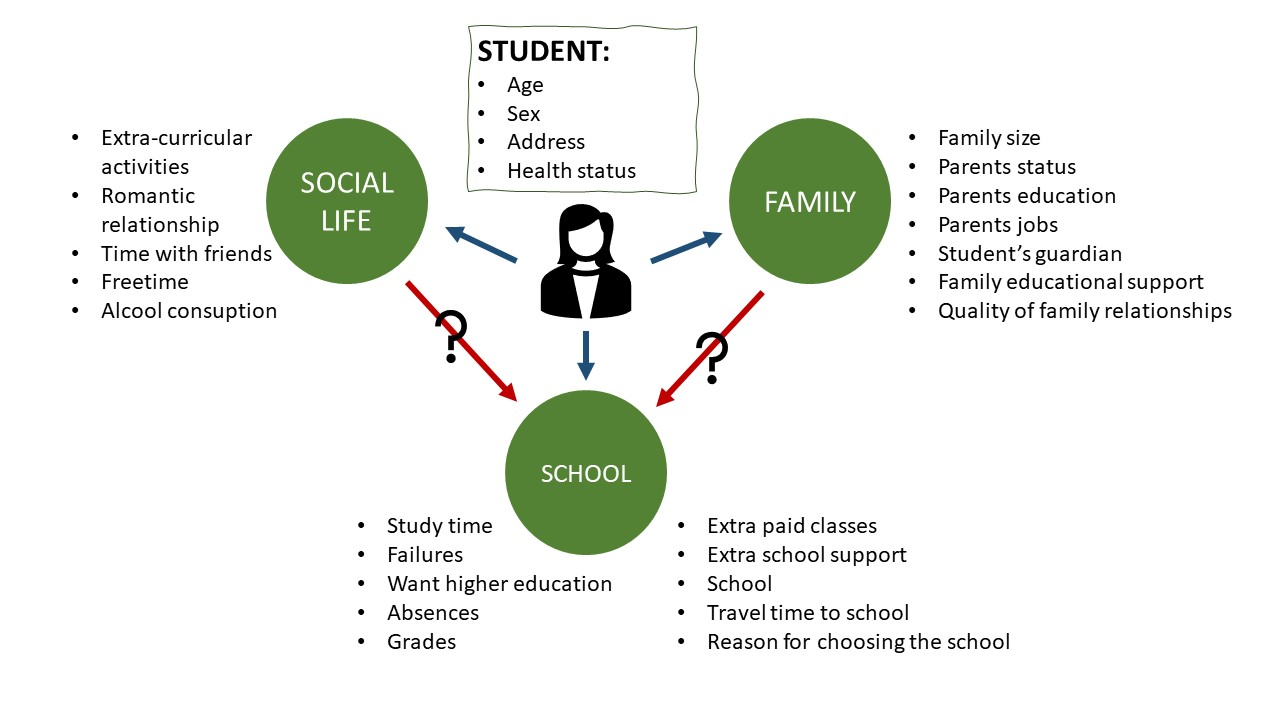
\includegraphics[scale=0.4]{variables.jpg}
\caption{Dataset variables associated with their macroarea.}
\end{figure}

\\After a first glance at the dataset these three variable subsets caught our eyes. In our opinion families and social life impact children's academic path in some way. There are many studies that show how parents with higher educational level have most likely children with higher grades or that want higher education. As the same time, we expect that someone who attends many extra-curricular activities and spend lots of time with friends has less time to study and therefore lower grades. 
\\In this project we want to study the data in order to see if we can credit our opinions or not and to try to predict grades knowing all the other variables. For doing that we want to use statistical visualisations and statistical testing in order to give a more accurate and precise point of view of the analysis .


\flushleft
\noindent
\begin{figure}\makebox[1 \textwidth][c]{       %centering table
\resizebox{1.3 \textwidth}{!}{   %resize table
\begin{tabular}{ |p{2cm}|p{13cm}| }
\hline
Attributes &  Values\\
\hline
school & student's school (binary: "GP" - Gabriel Pereira or "MS" - Mousinho da Silveira)\\
\hline
sex & student's sex (binary: "F" - female or "M" - male)\\
\hline
age & student's age (numeric: from 15 to 22)\\
\hline
address & student's home address type (binary: "U" - urban or "R" - rural)\\
\hline
famsize & family size (binary: "LE3" - less or equal to 3 or "GT3" - greater than 3)\\
\hline
Pstatus & parent's cohabitation status (binary: "T" - living together or "A" - apart)\\
\hline
Medu & mother's education (numeric: 0 - none,  1 - primary education (4th grade), 2 – 5th to 9th grade, 3 – secondary education or 4 – higher education)\\
\hline
Fedu & father's education (numeric: 0 - none,  1 - primary education (4th grade), 2 – 5th to 9th grade, 3 – secondary education or 4 – higher education)\\
\hline
Mjob & mother's job (nominal: "teacher", "health" care related, civil "services" (e.g. administrative or police), "at_home" or "other")\\
\hline
Fjob & father's job (nominal: "teacher", "health" care related, civil "services" (e.g. administrative or police), "at_home" or "other")\\
\hline
reason & reason to choose this school (nominal: close to "home", school "reputation", "course" preference or "other")\\
\hline
guardian & student's guardian (nominal: "mother", "father" or "other")\\
\hline
traveltime & home to school travel time (numeric: 1 - <15 min., 2 - 15 to 30 min., 3 - 30 min. to 1 hour, or 4 - >1 hour)\\
\hline
studytime & weekly study time (numeric: 1 - <2 hours, 2 - 2 to 5 hours, 3 - 5 to 10 hours, or 4 - >10 hours)\\
\hline
failures & number of past class failures (numeric: n if 1<=n<3, else 4)\\
\hline
schoolsup & extra educational support (binary: yes or no)\\
\hline
famsup & family educational support (binary: yes or no)\\
\hline
paid & extra paid classes within the course subject (Math or Portuguese) (binary: yes or no)\\
\hline
activities & extra-curricular activities (binary: yes or no)\\
\hline
nursery & attended nursery school (binary: yes or no)\\
\hline
higher & wants to take higher education (binary: yes or no)\\
\hline
internet & Internet access at home (binary: yes or no)\\
\hline
romantic & with a romantic relationship (binary: yes or no)\\
\hline
famrel & quality of family relationships (numeric: from 1 - very bad to 5 -excellent)\\
\hline
freetime & free time after school (numeric: from 1 - very low to 5 - very high)\\
\hline
goout & going out with friends (numeric: from 1 - very low to 5 - very high)\\
\hline
Dalc & workday alcohol consumption (numeric: from 1 - very low to 5 - very high)\\
\hline
Walc & weekend alcohol consumption (numeric: from 1 - very low to 5 - very high)\\
\hline
health & current health status (numeric: from 1 - very bad to 5 - very good)\\
\hline
absences & number of school absences (numeric: from 0 to 93)\\
\hline
G1 & first period grade (numeric: from 0 to 20)\\
\hline
G2 & second period grade (numeric: from 0 to 20)\\
\hline
G3 & final grade (numeric: from 0 to 20, output target)\\
\hline
\end{tabular}
}
}
\caption{\label{fig:text3}Variables meaning}
\end{figure}


We also decide to split our work in four different points answering different questions:
\begin{enumerate}
\item What's the correlation between variables?
\item Do the grades follow a normal distribution ?
\item Which is the capacity of different variables to explain the grades ?
\item Can we train a model to predict grade based on the other variables ?
\end{enumerate}
and for each point we used different statistical methods.


\section*{1. Correlations and Hypothesis testing}
In this part we study if there's any correlations between variables, for doing that we calculated Pearson correlation coefficient that measures linear correlation between two sets of data.

\begin{itemize}
\item \textbf{Correlation between Study time and Grades}
\\Before running the calculation our $a$ $priori$ estimation was that the time of studying influences the grades in a positive way, in theory the more you study the more you succeed in tests. Oppositely, the less you study the more you fail at tests. So, analysing the $r$ coefficient, we got these results:
\begin{center}
\begin{tabular}{|p{3cm}|p{4cm}|p{4cm}|}
 & Grades & Failures\\
\hline
$r$ coefficient & $0.249788689998863$ & $-0.14744054515158145$\\
\hline
Standard error & $0.036861080126113825$ & $0.03845941964984769$\\
\hline
\end{tabular}
\end{center}

As we expected there's a positive correlation between Study time and Final grades, and a negative correlation between Study time and Failures. However, the value of the coefficient in both cases is pretty low, so it doesn't seem to be a great correlation between the two. 

\begin{figure}[h]\centering
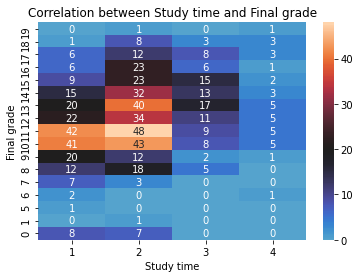
\includegraphics[scale=0.42]{g3-st.png}\quad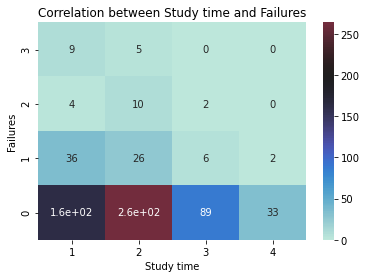
\includegraphics[scale=0.42]{failures.png}
\caption{Study times - Final grades and Failures.}
\end{figure}

In the above figure we can observe two heatmaps describing the correlations we've just studied. The higher is the color in the scale the higher is the amount of students with a certain match 'final grade'-'study time'.


\item \textbf{Correlation between Sex and academic performances}
\\For the gender correlation we didn't have precise $a$ $priori$ estimations because apparently there's no need to think that belonging to a particular gender can affect grades.

\begin{figure}[h]\centering
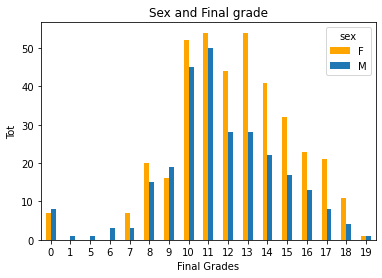
\includegraphics[scale=0.44]{sexgrades.png}\quad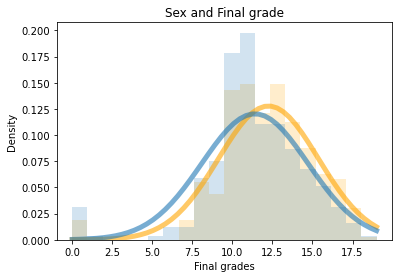
\includegraphics[scale=0.44]{distrib.png}
\caption{Correlation between Gender and Final grades, considering that the total of female is $383$ and the total of males is $266$.}
\end{figure}

The first figure shows that there are more males with lower grades than females and that the grade mean for female is higher than the one for males. At this point we should look if there is any remarkable relationships with the Study time.

\begin{figure}[h]\centering
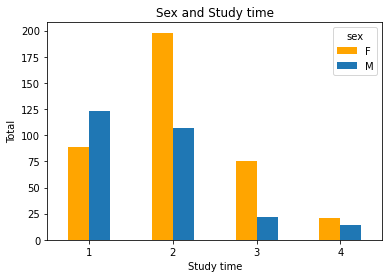
\includegraphics[scale=0.44]{sexstudy.png}
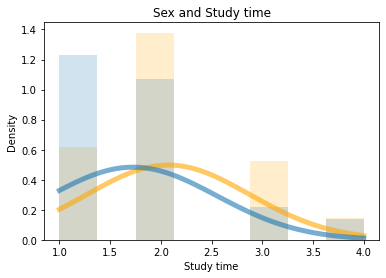
\includegraphics[scale=0.44]{distrib2.png}
\caption{Correlation between Gender and Study time, considering that the total of female is $383$ and the total of males is $266$.}
\end{figure}

In the second graphic we can see that the density of men having the value $1$ (the lowest one) of study time is way higher than the girls one. However, for higher value of study time the female density is higher than the males one. We can say that on average males study less than females and, as a consequence, on average they also have lower grades.



\item \textbf{Correlation between age and Final grade}
\\Another question could be if the students age can have some consequences on the grades they get. Our $a$ $priori$ expectation was that there is no correlation between the two because each year students have to study subjects appropriate for they ages . We calculated the Pearson's correlation coefficient and obtained:
\begin{center}
\begin{tabular}{|p{3cm}|p{4cm}|}
$r$ coefficient & $-0.008415114730320437$ \\
\hline
Standard error & $0.0393112727067965$ \\
\hline
\end{tabular}
\end{center}
\\The $r-$coefficient is negative and overall is really low, so it credits our idea of non correlation between age and Final grades. The heatmap below shows the relationships between the two of them.

\begin{figure}[h]\centering
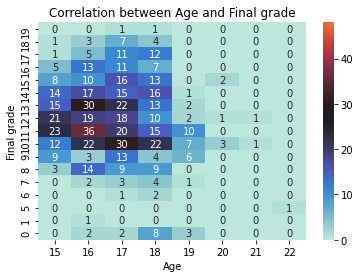
\includegraphics[scale=0.45]{age.png}
\caption{Correlation between Age and Final grades.}
\end{figure}


\item \textbf{Correlation between Student family and grades}
\\We now study how the family environment impacts on the students academic performances. First we analyse the family size. In the graphic below we compared student with families larger than three people and the ones equal or smaller than three people.

\begin{figure}[h]\centering
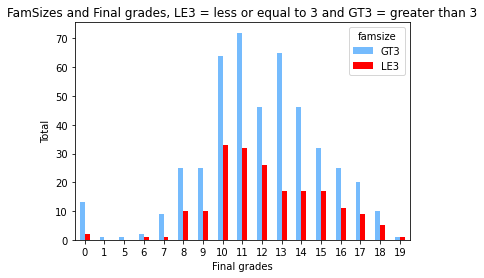
\includegraphics[scale=0.44]{famsize.png}\quad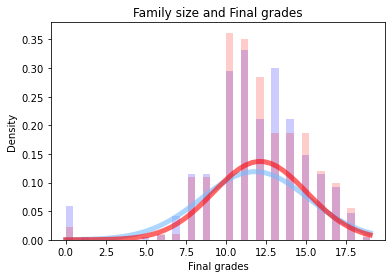
\includegraphics[scale=0.44]{distrib3.png}
\caption{Correlation between Family size and Final grades, considering that the total of family with less than three people is $192$ and the total of the other ones is $457$.}
\end{figure}
We can notice that the mean of grades for students with big family is a bit lower than the one for small family. Furthemore, in higher grades students with small families have higher density than the other ones.

We believe that parents living together can affect students grades in a positive way, probably because a compacted family may create a less stressfull environment for students and therefore can get to higher grades.
\begin{figure}[h]\centering
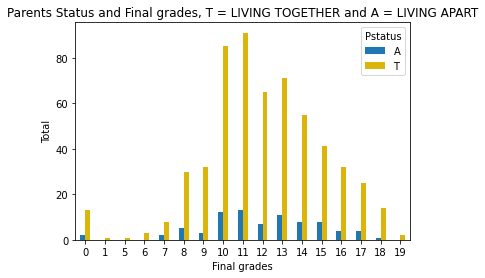
\includegraphics[scale=0.44]{pstatus.png}\quad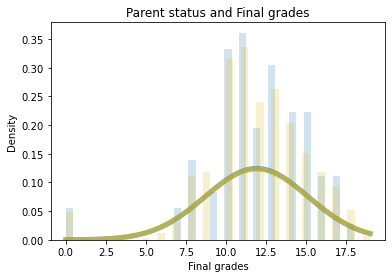
\includegraphics[scale=0.44]{distrib4.png}
\caption{Correlation between Parents status and Final grades considering that that total amount of students with parents living together is 569 and for the other ones is 80.}
\end{figure}

In the figure above we can notice that then mean of grades for students with parents living together and the one with parents living apart is the same. In this case there is no relevant difference between the two density so in this case if parents are separated or not doesn't affect their children grades.
\\As we said, we believe that good family relationship can affect students grades in a positive way.
Now we verify the Pearson's correlation coefficient between Family relationships and Final grades:
\begin{center}
\begin{tabular}{|p{3cm}|p{4cm}|}
$r$ coefficient & $0.06336112772983048$ \\
\hline
Standard error & $0.03915622520852588$ \\
\hline
\end{tabular}
\end{center}
Once again the data analysis destroys our $a$ $priori$ expectation, in fact we found a very low correlation coefficient that shows that quality of family relationships doesn't affect students grades.

\begin{figure}[h]\centering
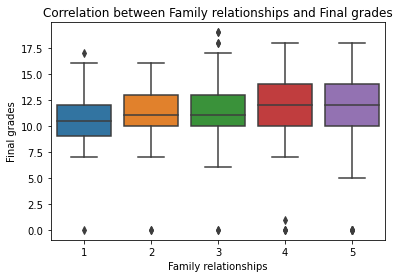
\includegraphics[scale=0.5]{famrel.png}
\caption{Correlation between Family relationships and Final grades.}
\end{figure}


In the figure below we show a summary graphic for the correlation between Family and Final grades.
\begin{figure}[h]\centering
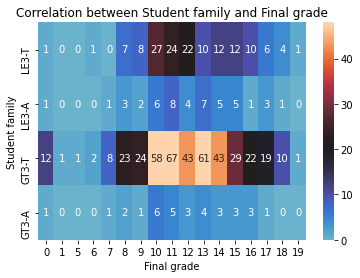
\includegraphics[scale=0.5]{family.png}
\caption{Correlation between Family environment and Final grades.}
\end{figure}



\end{itemize}




\section*{2. normality of final grades}

To understand whether variable G3 has normal distribution we used different
techniques. Firstly we tried to plot an histogram with the distribution of the variable. Then over the histogram we plotted a line-plot of a gaussian with same mean and same variance as the variable.

\begin{figure}[h]
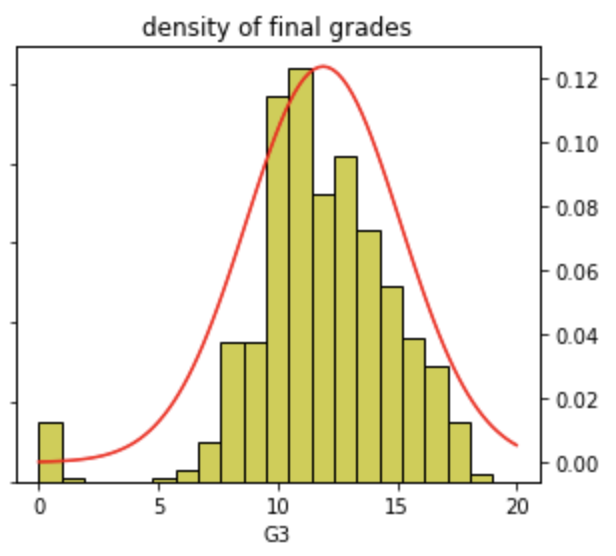
\includegraphics[scale=0.5]{G3_distribution.png}
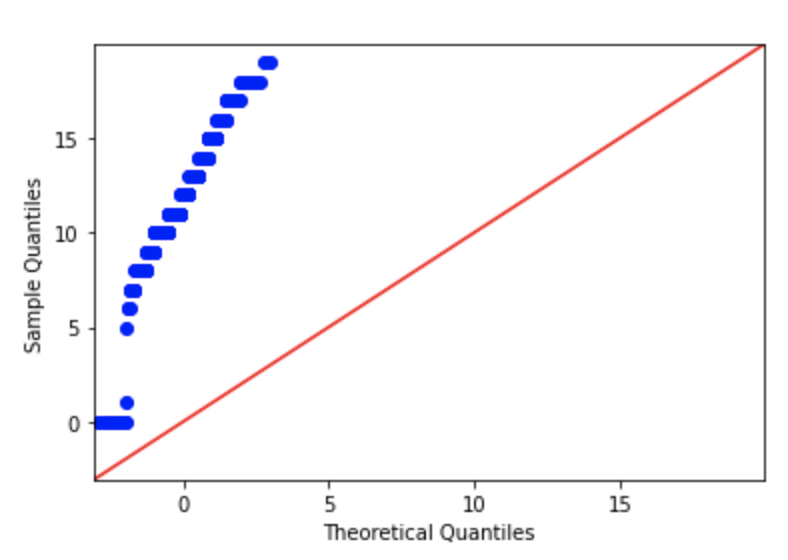
\includegraphics[scale=0.5]{qq-plot_G3.png}
\caption{comparing normal distribution with G3 histogram and qq-plot}
\end{figure}

As we can notice from the first plot we can already think that the distributions of the variable is not normal. In fact G3 has too many data in the tails, which underline that it must not be normal.

Just to be sure that our data are actually not normal we then apply more quantitative tests: QQ-plot and Shapiro-Wilks test.
The results make clear that the three distributions can't be normal, in fact the p value of Shapiro test are smaller than 10e-17, which give no evidence to accept the null hypothesis. The QQ-plots then confirms that we can't believe that the three distributions are normal.

We also tried to understand whether it can be normal without the outliers, but again the Shapiro test has a really small p value: 10e-6.

\section*{3. Grades}


\section*{4. Machine Learning}

All the models have been trained with a 80 to 20 percentage split for training to testing and implemented using the Sklearn library.

\subsection*{Baseline}
The baseline is a constant prediction model which outputs always the most frequent class ( in our dataset is 11 ), this achieves an accuracy of 16 percent.
\subsection*{Logistic Regression}
Logistic regression is a statistical model that in its basic form uses a logistic function to estimate the probabilities for a multivariate dependent variable: $$p=\frac{1}{1+b^{-\left(\beta_{0}+\beta_{1} x_{1}+\beta_{2} x_{2}+\cdots+\beta_{m} x_{m}\right)}}$$
Our model with L2 loss and balanced weights achieved an accuracy of 10.7 percent. 
\subsection*{Random Forest}
Random forests are an ensemble learning method, used for classification in this case, that operates by constructing a multitude of decision trees at training time and correct for decision trees' habit of overfitting to their training set. Our model with max depth of a tree equal to 2 achieved an accuracy of 12.3 percent.
\subsection*{XGboost}
XGboost is a gradient boosting is a machine learning technique, used for classification in this case, which produces a prediction model in the form of an ensemble of weak prediction models, typically decision trees. In particular XGboost is also connected to the Newton-Raphson method. Our model with max depth of a tree equal to 3 achieved an accuracy of 23.8 percent.

\section*{4. Machine Learning}
The aim of the Machine Learning section is to apply some of the most popular Machine Learning techniques to our dataset in order to generalise relevant information contained in the dataset.
The easiest and first question which we want to address is the following:
\begin{itemize}
\item \textit{Can we build a model which can predict the final grade G3 based on the other features ?}
\end{itemize}
To answer this question we tried different models and we compared their performances. First of all, we preprocessed the data. Indeed, as we can see from the table above (which contains the information of the dataset) our original dataset is made of discrete and categorical features. For instance, the attribute 'address' is categorical because it can be 'U' for urban and 'R' for rural so it can belong to two distinct classes and there is no ordering relationship between the classes. However, we have also some variables which assume discrete range of values like 'age' which is a number from $15$ to $22$ or 'G1' which is an integer from $0$ to $20$. The first thing that we need to do is saving the dataset in a pandas dataframe and then perform one hot encoding on categorical variables. Indeed, for each categorical variable $v$ assuming values in a set $S$ with $S=\{s_1,s_2,\dots, s_k\}$, we create $k$ new columns and for each row we set the n-th created column equal $1$ if and only if in the original column v assumed the value $s_n$, we set it to zero otherwise, we finally delete the original column. In this way we are mapping each value $s_i$ to a vector with $k$ components whose i-th component is equal to one and the other components are equal to zero. This is a common technique in Machine Learning because it allows to encode categorical values in numerical values on the top of which we can train our machine learning model. Then we plot the correlation matrix to discover which variables are the most correlated to the output we would like to predict (G3). The result is shown below. 
\begin{figure}[h]\centering
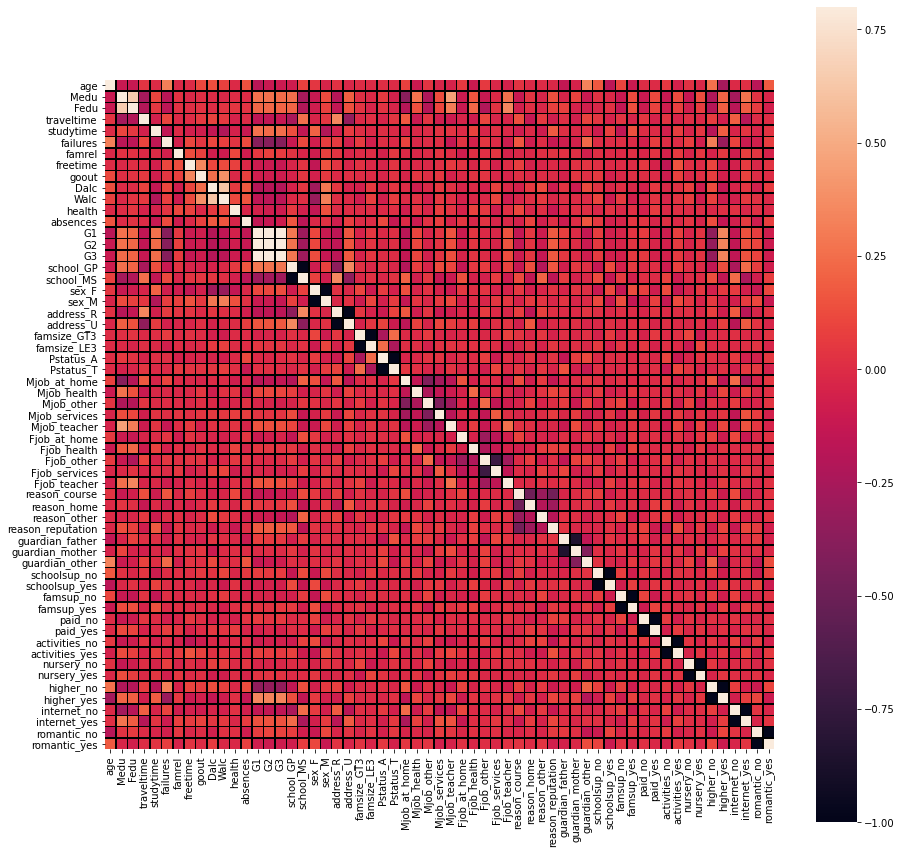
\includegraphics[scale=0.4]{heatmap.png}
\caption{Correlation between the variables of the preprocessed dataset}
\end{figure}
As we can easily observe, there is a high correlation between G3 and G1, G2, we have a low but significant positive correlation between G3 and the study time, the mother and father education and the desire of pursuing a higher education. On the other hand we have a negative correlation between G3 and the number of failures, the number of workday/weekend alchool consumption and the desire not to pursue a higher education. All this information are exactly what we would have expected. Then we split the data in $X$, a matrix containing all the features a part from G3 and $Y$ a column vector containing just the G3 feature. We then split each of them in $X_{\text{train}}$, $X_{\text{test}}$, $Y_{\text{train}}$, $Y_{\text{test}}$. We will use $X_{\text{train}}$ and $Y_{\text{train}}$ to train our model and then we will evaluate the performance using $X_{\text{test}}$ and $Y_{\text{test}}$. To answer this question we have considered the problem as a regressive problem and we have used the following models/approaches. All the models have been trained with a 80 to 20 percentage split for training to testing and implemented using the Sklearn and Keras library. To determine if a model is non trivial we compare it against a baseline, which is a constant prediction model which outputs always the most frequent class ( in our dataset is 11 ), this achieves an accuracy of 16 percent.
\begin{enumerate}
    \item We used a dense Neural Network with 7 layers with a large number of neurons for each layer. We used 'relu' as the activation function and we chose Adam as the optimizer. In addition to that, in order to prevent overfitting we applied the following early stopping technique. We have taken a subset of the training data as validation data and at the end of each epoch we computed the loss that the current model would have had on the validation data and we have saved the model corresponding to the smallest validation loss. After we have trained our model, we applied the model to $X_{\text{test}}$ in order to obtain the predictions corresponding to $Y_{\text{test}}$ we then have rounded the predictions because G3 has to be an integer value between 0 and 20. We computed the Mean Squared Error between the predicted and the ground-truth grades and we have obtained a value of $1.94$. This information is not enough for us to understand if the model made a good fit or not for G3. Therefore, we tried to visualise the results obtained.
    This is how our results look like compared to the real grades.
    \begin{figure}[h]\centering
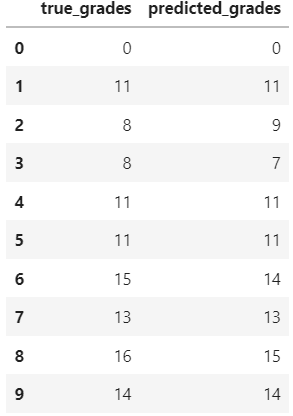
\includegraphics[scale=0.4]{predictions G3 neural nets using all features.PNG}
\end{figure}
As we can see from the first 10 students the predictions are quite accurate, however we cannot really understand how good the predictions are just comparing the true grades and the predicted grades with a table. We will now use different plots to have a better perspective of the fit. The first plot is a scatter plot of the true and predicted grades.
    \begin{figure}[h]\centering
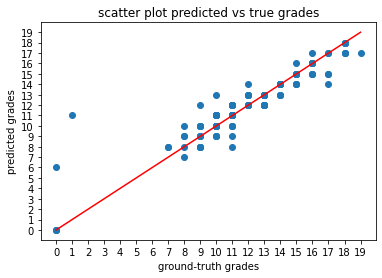
\includegraphics[scale=0.4]{scatter plot G3 neural nets using all features.png}
\end{figure}
We would expect the points to be on the line y=x since our predicted grades should be equal to the true grades. As we can see from the plot this is indeed true but of course not all the points lie on the line and some variance around the line is observed. We then used the following line plot to compare the predictions with the true grades for the first 20 students.
    \begin{figure}[h]\centering
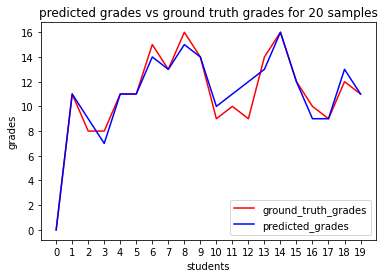
\includegraphics[scale=0.4]{plot G3 neural nets using all features.png}
\end{figure}
Again we observe that the predictions are quite accurate.
All this plots suggested a good fit but in order to confirm our hypothesis we have used the Kolmogorov-Smirnov test for goodness of fit. Having as a null hypothesis that the distributions of the true grades and the one of the predicted grades were the same distribution we obtained a very large p-value suggesting us that we cannot reject the null hypothesis and consequently that our fit is a good one.
\item As a second model we have used the support vector machine for regression. We have tuned the hyperparameters of the model using grid-search trying out different kernels, degree and coefficients. This model showed a worse performance compared to neural nets, indeed the Mean Squared Error in this case turned out to be $2.11$. The plots reflect the drop in performance.
\newline
    \begin{frame}
      \centering
        \begin{tabular}{c}
         \\
        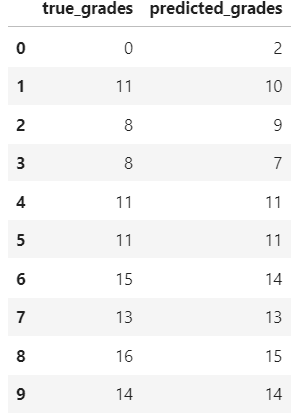
\includegraphics[width=4cm]{predictions G3 SVR using all the features.PNG}
      \end{tabular}

      \vspace{0.05em}
        \begin{tabular}{cc}
          &  \\
        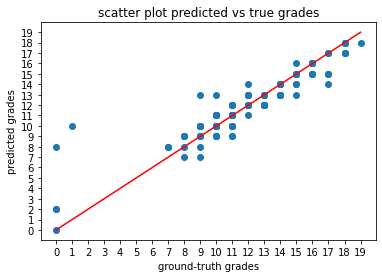
\includegraphics[width=4cm]{scatter plot G3 SVR using all the features.png}
         &
         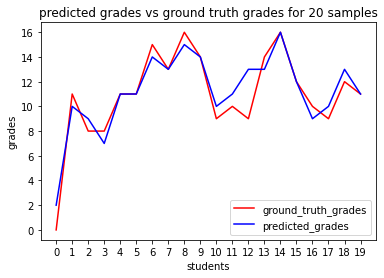
\includegraphics[width=4cm]{plot G3 SVR using all features.png}
         \end{tabular}
    \end{frame}
\newline
However, in this case too, we cannot reject the null hypothesis that the predicted grades and the true grades come from the same distribution using Kolmogorov-Smirnov test for goodness of fit.
\newline
\item To further increase the performance we can now train the neural net model on the same dataset but preprocessed such that no outliers are now present in the dataset. In this case we reach a mean squared error of 0.22 and as we can see the predicted grades are almost always correct.
\newline
    \begin{frame}
      \centering
        \begin{tabular}{c}
         \\
        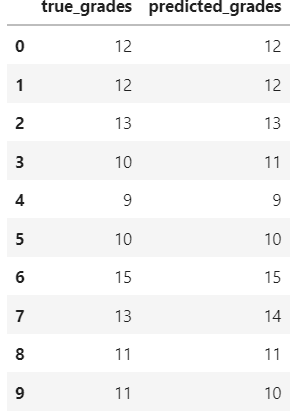
\includegraphics[width=4cm]{predictions G3 neural nets no outliers.PNG}
      \end{tabular}

      \vspace{0.05em}
        \begin{tabular}{cc}
          &  \\
        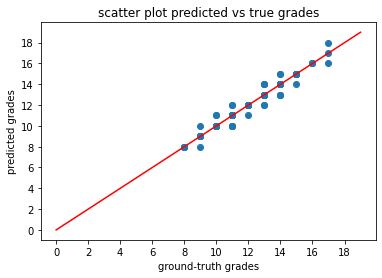
\includegraphics[width=4cm]{scatter plot G3 neural nets no outliers.png}
         &
         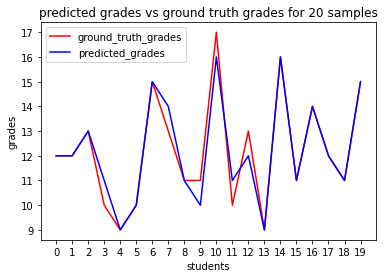
\includegraphics[width=4cm]{plot G3 neural nets no outliers.png}
         \end{tabular}
    \end{frame}
\newline
Clearly also in this case we cannot reject the null hypothesis of the Kolmogorov-Smirnov test for goodness of fit having a p-value of $0.9999999$.
\item We also tried out two model that obtained mediocre results, logistic regression which is a statistical model that in its basic form uses a logistic function to estimate the probabilities for a multivariate dependent variable: $$p=\frac{1}{1+b^{-\left(\beta_{0}+\beta_{1} x_{1}+\beta_{2} x_{2}+\cdots+\beta_{m} x_{m}\right)}}$$
Our model with L2 loss and balanced weights achieved an accuracy of 10.7 percent. Also random forests did not predict better than the baseline, they are an ensemble learning method, used for classification in this case, that operates by constructing a multitude of decision trees at training time and correct for decision trees' habit of overfitting to their training set. Our model with max depth of a tree equal to 2 achieved an accuracy of 12.3 percent.
\item Meanwhile a method that obtained a good result is XGboost, which is a gradient boosting technique, used for classification in this case, which produces a prediction model in the form of an ensemble of weak prediction models, typically decision trees. The idea behind gradient boosting algorithm is to build and increasingly better estimator considering a sequence of weak learners, of fixed size, and try to fix the error of the preceding learner with a new learner. Our model with max depth of a tree equal to 3 achieved an accuracy of 23.8 percent.
\end{enumerate}
In the last two models we took a different interpretation of the problem than the first three, in fact the problem was posed as a multi-classification problem on the finite set of possible grades G3, therefore on those it was possible to calculate an accuracy score and not a MSE as we obtained for the regression interpreted models.
As we have seen our models work quite well and we can be satisfied of the reached fit. The next questions that might arise spontaneously is the following
\begin{itemize}
    \item \textit{Can we train a model which can predict the final grade G3 based on all the other features except the previous grades G1 and G2 ?}
\end{itemize}
We have tackled this question training the neural net model on a new $X'_{\text{train}}$ which is exactly the same as the $X_{\text{train}}$ described before a part from the column related to G1 and G2 which are not present in $X'_{\text{train}}$. The same applies to $X'_{\text{test}}$. We followed the exact same procedure described in the answer to the previous question but in this case we have reached a mean squared error of just $11.02$. The following plots testify this poor results.
\newline
    \begin{frame}
      \centering
        \begin{tabular}{c}
         \\
        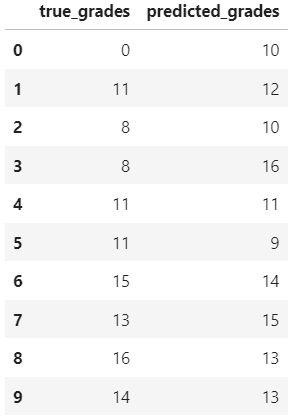
\includegraphics[width=4cm]{predictions G3 without G1 and G2.PNG}
      \end{tabular}

      \vspace{0.05em}
        \begin{tabular}{cc}
          &  \\
        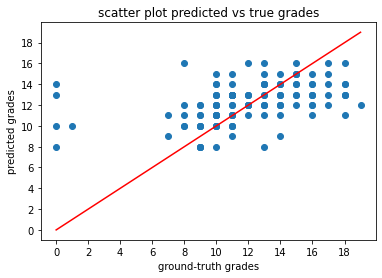
\includegraphics[width=4cm]{scatter plot G3 without G1 and G2.png}
         &
         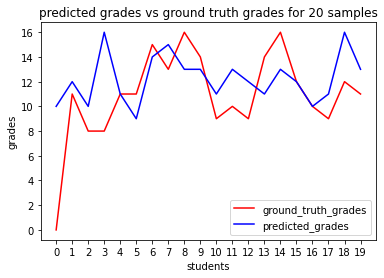
\includegraphics[width=4cm]{plot G3 without G1 and G2.png}
         \end{tabular}
    \end{frame}
\newline
As we can see from the scatter plot there is a high variety in the difference between the predictions and the true grades and how can we see in the line plot this drives to a poor fit. Also the Kolmogorov-Smirnov test notice the poor fit and now the p-vaue for the null hypothesis is only $0.067$. This does not indicate that we should reject the null hypothesis (with a significance level $\alpha = 0.05$) but it is an indicator of the poorness of the fit (since the p-value is quite small).
We could justify the results using the correlation matrix plotted before. Indeed, how we can see, G3 are highly positive correlated with G1 and G2 so, removing this two information, the model cannot predict G3 as well as before.
The next question that we are going to address is the following:
\begin{itemize}
    \item \textit{Can we predict the studytime based on the other features of the dataset ?}
\end{itemize}
We are going to answer to this question using a neural network based model since the best results obtained in the previous tasks were reached with this model. Obviously in this case after having split the dataset in training and test, $Y_{\text{train}}$ will be just the column related to the studytime and $X_{\text{train}}$ the columns for all the other features. The same applies to $X_{\text{test}}$ and $Y_{\text{test}}$. In this case when we apply the model to $X_{\text{test}}$ creating the prediction and when we compare them with $Y_{\text{test}}$ we have the following results.

\begin{figure}[h]\centering
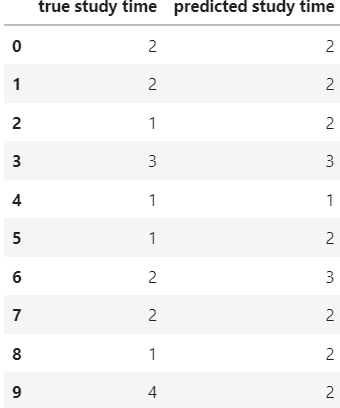
\includegraphics[scale=0.4]{prediction study time neural nets.PNG}
\end{figure}
    \begin{figure}[h]\centering
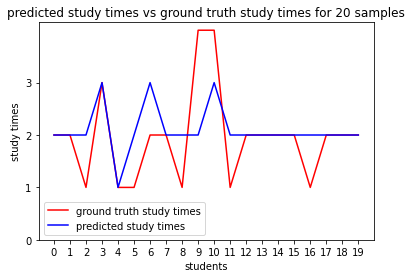
\includegraphics[scale=0.4]{plot study time neural nets.png}
\end{figure}

We have obtained another poor fit testified by a really small p-value in Kolmogorov-Smirnov test (0.0042). The reason why we have such a bad fit lies probably on the fact that we do not have enough data correlated with the feature 'studytime'. Indeed, the dataset was collected to explain the grades of the students and not their studytime. As a direct consequence, despite the model we use to predict the studytime, we will never have a good fit due to the lack of crucial missing variables such as the time that students spend at home or in different other activities.
The last question that we would like to give an answer to is the following:
\begin{itemize}
    \item \textit{Can we predict whether a student is in a romantic relationship or not based on the other features of the dataset?}
\end{itemize}
We have used three different models to answer to this question.
\begin{enumerate}
    \item A first method based on dense neural networks which scored $0.62$ in accuracy
    \item A second method based on Support Vector Machine tuned with grid-search which scored $0.65$ in accuracy 
    \item A third model based on Logistic Regression tuned with grid-search which scored $0.65$ in accuracy.
\end{enumerate}
Recalling the definition of accuracy:
\begin{align*}
    \text{accuracy} = \frac{\text{number of correctly classified samples}}{\text{number samples}}
\end{align*}
we notice that an accuracy around $0.65$ is not high at all. Since we tried different models and we have always tuned the hyperparameters, we can claim that the problem lies in the lack of crucial variables as happened in the studytime analysis. Indeed, as we can observe from the correlation matrix, there are not highly positive or highly negative correlated variables with the romantic relationship variable.



\end{document}
